\section{Motivation}

In this section, we first study the typical shuffle characteristics (\ref{shuffle pattern}), and then spot the opportunities to achieve shuffle optmization (\ref{observation})
\subsection{Characteristic of Shuffle} \label{shuffle pattern}

In large scale data parallel computing, enormous datasets are partitioned into pieces to fit into the memory of each node.
Meanwhile, complicated application procedures are divided into steps. The succeeding steps take the output of ancestors as computation input. Shuffle occurs when each successor needs 
part of data from all ancestors' output. It is designed to achieve an all-to-all data blocks transfer among nodes in the cluster. It exists in both MapReduce models and DAG computation models.
For clear illustration, we define those computing on each partition of data in one step as a \textit{task}. 
Those tasks that generate shuffle outputs are called as \textit{map} tasks, and tasks consuming shuffle outputs are called as \textit{reduce} tasks.
% Note that one task may have both shuffle data generation and consumption in modern DAG framework. These tasks contain characteristic of both map task and reduce task. But these tasks won't change the behavior of shuffle. To avoid ambiguity, in the following paper, we will only use term of map task to represent those who produce shuffle output, and reduce task to represent those who consume shuffle output.

\textbf{Overview of shuffle process}. As shown in Figure \ref{fig:shuffle_process}, shuffle mainly contains two phases itself: \textit{data partition} and \textit{data transfer}. For \textit{data partition}, each map task will partition the result data (key, value pair) after execution ("Execution" block in Figure \ref{fig:shuffle_process}) into several buckets according to the partition function.
The total number of buckets equals to the number of tasks in the next step. 
\textit{Data Transfer} can be further divided into two parts: \textit{shuffle write} and \textit{shuffle read}. \textit{Shuffle write} starts after data partition ("Data Partition" block in Figure \ref{fig:shuffle_process}) of map tasks. 
During \textit{shuffle write}, all the partitioned shuffle output data will be written into local persistent storage for fault tolerance  \cite{mapreduce, spark}.
\textit{Shuffle read} starts at the beginning of reduce tasks. These tasks might fetch the data that belong to their corresponding partitions from both remote nodes and local storage.

%In short, shuffle is loosely coupled with application context and it's I/O intensive.

\textbf{Impact of shuffle process}. Shuffle process is I/O intensive, which might can introduce a significant latency to the application. Reports show that 60\% of MapReduce jobs at Yahoo!
and 20\% at Facebook are shuffle intensive workloads \cite{shufflewatcher}. For those shuffle intensive jobs, the shuffle latency may even dominate Job Completion Time (JCT). 
For instance, a MapReduce trace analysis from Facebook shows that shuffle accounts for 33\% JCT on average, up to 70\% in shuffle intensive jobs \cite{managing}.
% Besides, the completion time of shuffle correlates with the performance of storage devices, network and even applications. 
% This variation may bring a huge challenge for operators to find the correct configuration of the DAG framework.
\begin{figure}
	\centering
	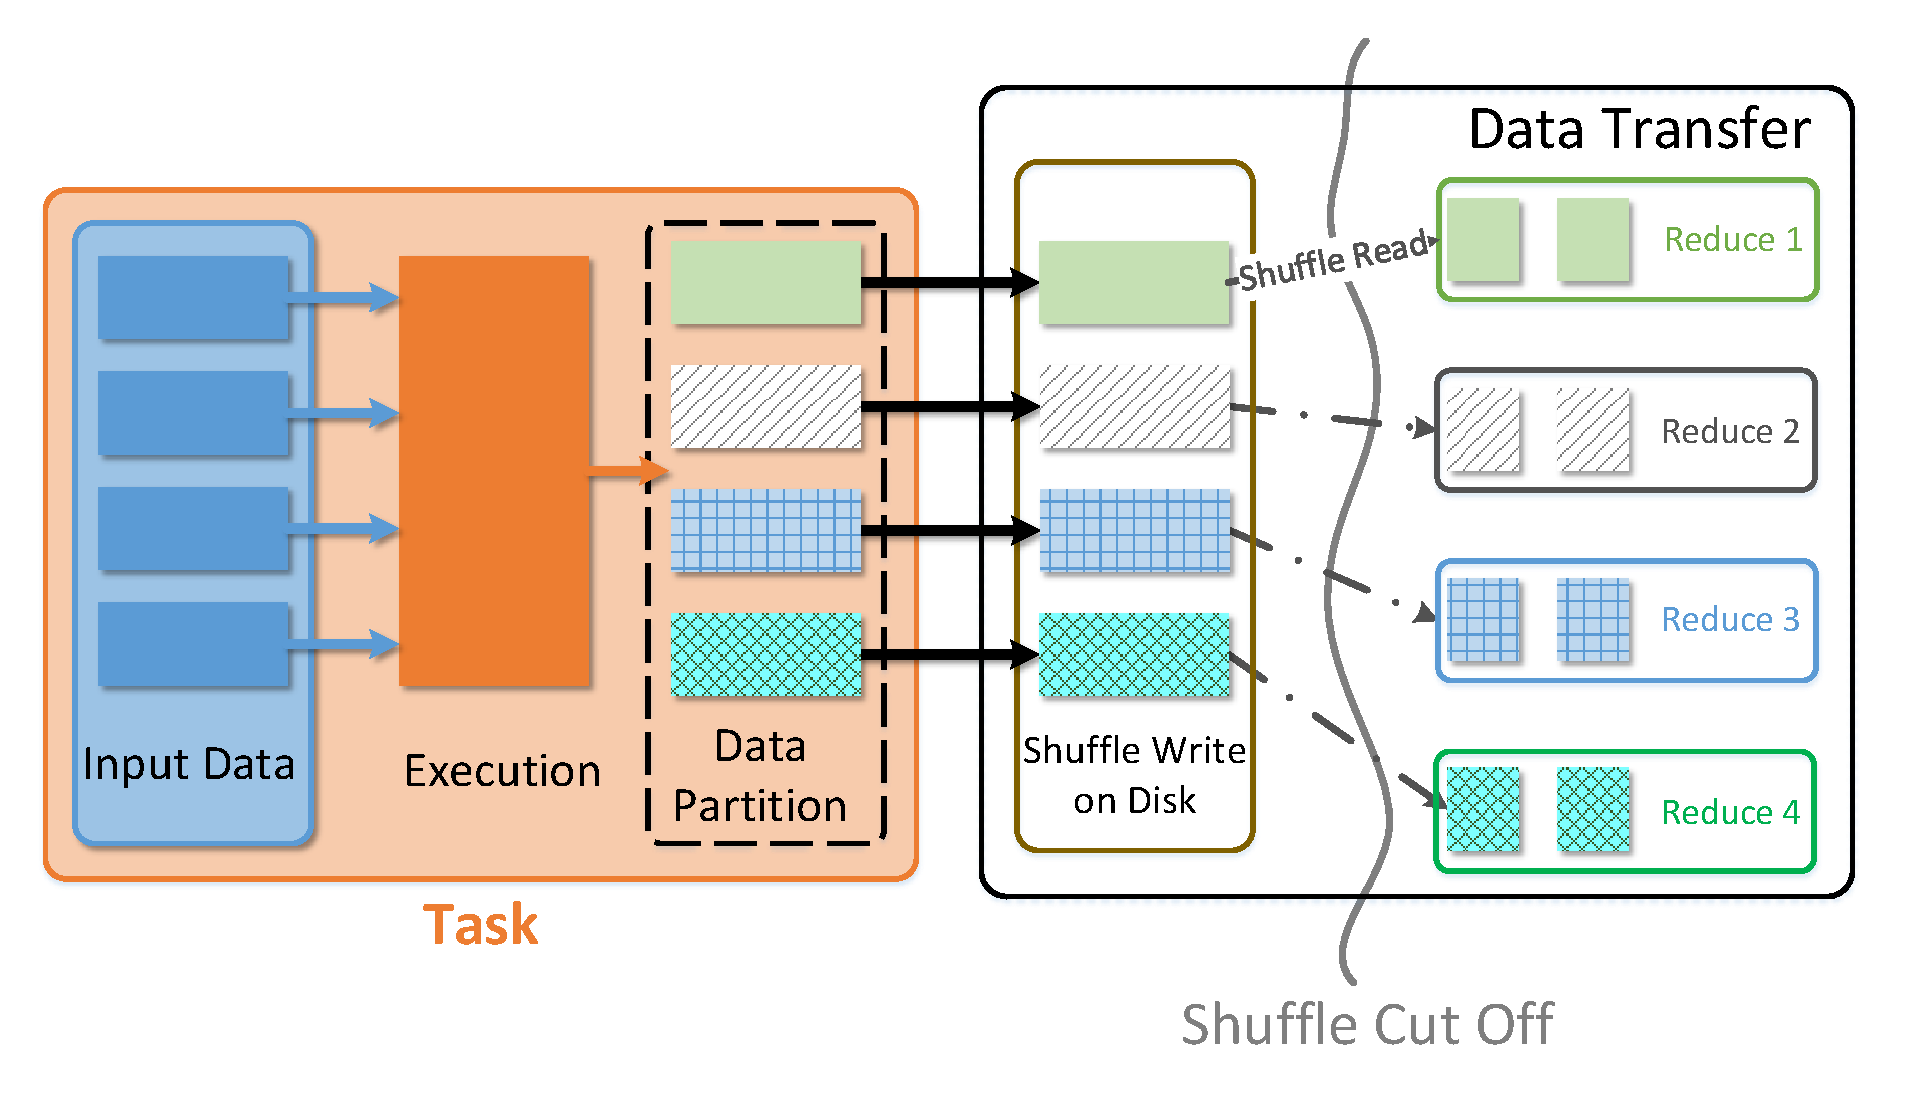
\includegraphics[width=\linewidth]{fig/shuffle_process}
	\caption{Shuffle Overview}
	\label{fig:shuffle_process}
\end{figure}

\subsection{Observations} \label{observation}
Of course, shuffle is unavoidable in a DAG computing process. But can we mitigate or even remove the overhead of shuffle? To find the answers, we run some typical Spark applications in a 5-node EC2 cluster with \texttt{m4.xlarge}. We then measure the CPU utilization, I/O throughput and tasks execution information of each node. Here we present the trace of one node running Spark \textit{GroupByTest} in Figure \ref{fig:util} as an example. This job has 2 rounds of tasks for each node. 
We have marked out the \textit{execution} phase as from the launch time of the first task to the execution finish timestamp of the last one. The \textit{shuffle write} phase is marked from the timestamp of the beginning of the first partitioned data write. The \textit{shuffle read and execution} phase is marked from the start of the first reduce launch timestamp.

Figure \ref{fig:util} reveals the performance information of two stages that are connected by shuffle. By analyzing the trace combing with Spark source code \cite{sparksource}, we propose the following observations. 
% \begin{figure*}
% 	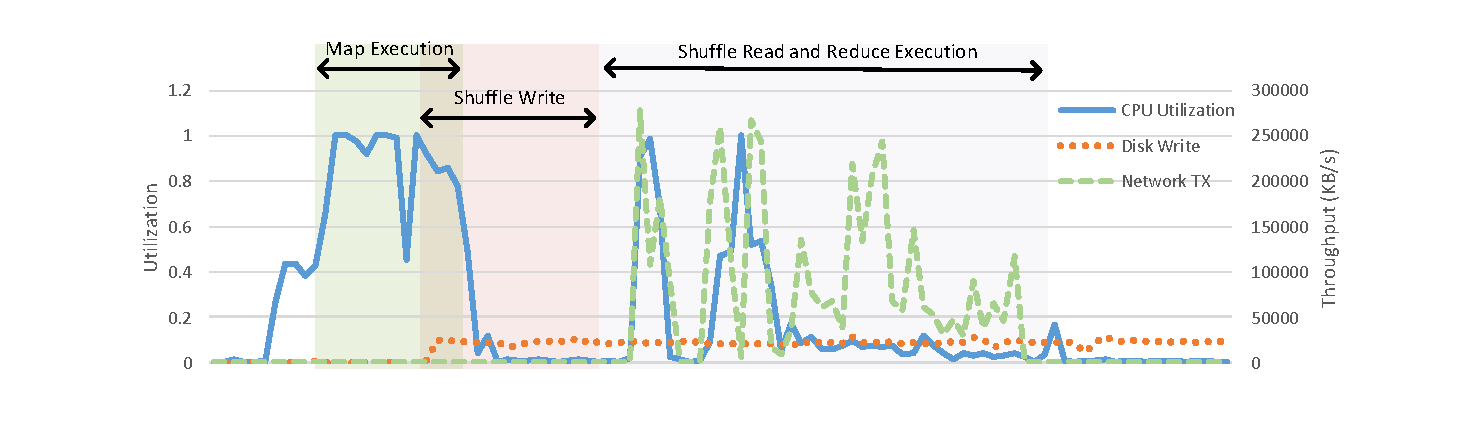
\includegraphics[width=\textwidth]{fig/util}
% 	\caption{CPU utiliazation and I/O throughput of a node during a Spark single shuffle application}
% 	\label{fig:util}
% \end{figure*}

\begin{figure}
	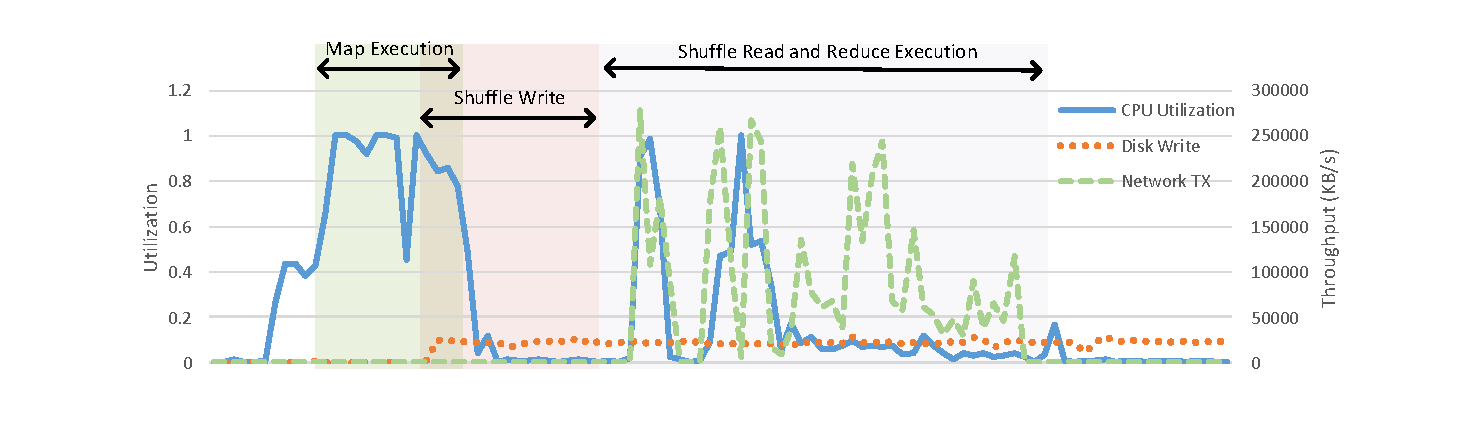
\includegraphics[width=\linewidth]{fig/util}
	\caption{CPU utilization and I/O throughput of a node during a Spark single shuffle application}
	\label{fig:util}
\end{figure}

\subsubsection{Coarse Granularity Resource Allocation}
In general, CPU and memory are bounded with a schedule slot in DAG resource scheduler. When a task is scheduled to a slot, it will not release the until the end of the task. In Figure \ref{fig:util}, the resource of Spark executor will be released at the ending of \textit{shuffle write}. On the reduce side, though in the context of Spark, the reduce task can do computation while fetching data, the transfer of first few blocks may still introduce an explict I/O delay. On the other hand, shuffle is an I/O intensive job without involving CPU. Both \textit{shuffle write} and \textit{shuffle read} occupy the slot without using CPU. The current coarse slot --- task mapping results in an inconsistency between resource demands and slot allocation, which further decrease the resource utilization. To break this inconsistency, a finer granularity resource allocation scheme must be provided.

\subsubsection{Synchronized Shuffle Read}
Combining with traces from other nodes, we find that almost all reduce tasks start \textit{shuffle read} simultaneously (i.e. The rising network utilization during \textit{shuffle read and execution} in Figure \ref{fig:util}). The synchronized \textit{shuffle read} requests cause a burst of network traffic. As shown in Figure \ref{fig:util}, the data transfer stresses on network bandwidth, which may result in network congestion among the cluster. This bursty demands of network bandwidth might delay the \textit{shuffle read} and hurt the performance of reduce stage. The previous work \cite{coflow, managing} also prove that the network transfer can introduce significant overhead in DAG computing.

\subsubsection{Multi-round Tasks Execution}\label{multi}
Both experience and DAG framework manuals recommend that multi-round execution of each stage will benefit the performance of applications.
For example, Hadoop MapReduce Tutorial  \cite{hadooptutorial} suggests that \textit{10-100 maps per-node} and \textit{0.95 or 1.75 $\times$ no. of nodes $\times$ no. of maximum container per node} seem to be the right level of parallelism. Spark Configuration also recommends 2-3 tasks per CPU core in the cluster \cite{sparkconf}.
In Figure \ref{fig:util} we also run two rounds of tasks to process data of about $70$GB. As shown in Figure \ref{fig:util}, during the map stage, the network is idle (i.e. Network utilization during \textit{execution} and \textit{shuffle write}). Since the shuffle data becomes available as soon as the execution of one map task is finished, if the destination of the shuffle output of each task can be known in priori, the property of multi-round can be leveraged to do \textit{shuffle read} ahead of reduce stage.


\subsubsection{Unefficient Persistent Storage Operation}
When we look into the detail I/O operations of shuffle, we find that the operations on persistent storage of shuffle are unefficient. There are at least two persistent storage operations for each shuffle data block. At first, Spark will write shuffle data to the persistent storage after map task execution(i.e. \textit{Shuffle Write} in Figure \ref{fig:util}). During the \textit{shuffle read}, Spark will then read shuffle data from remote and local presistent storage, which is the second operation. The persistence of shuffle data was designed for fault tolerance. But we believe it's not necessary for today's cluster. Recall that shuffle data only exist in a short time scale. But the Mean Time To Failure(MTTF) for a server is counted in the scale of year \cite{tachyon}, which is exponential comparing with the duration of a shuffle. In addition, the capacity of memory and network has been increasing rapidly in recent years. As a result, numbers of memory based distributed storage system have been proposed \cite{memcached, tachyon, ramcloud}. On the other hand, the size of shuffle data is relatively small. For example, shuffle size of Spark Terasort \cite{spark-tera} is less than 25\% of input data. The data reported in  \cite{makingsense} also shows that the amount of data shuffled is less than input data, by as much as 10\%-20\%. We argue that removing persistent storage and using memory to achieve shuffle fault tolerance is feasible and efficient.

Based on these observations, it is straightforward to come up with an optimization that uses memory to store the shuffle data and start \textit{shuffle read} ahead of reduce stage to overlap the I/O operations in \textit{multi-round} of DAG computing. To achieve this optimization:
\begin{itemize}
	\item Shuffle should be taken over to provide a fine granularity scheduling scheme.
	\item Reduce tasks should be pre-scheduled without launching to achieve shuffle data pre-fetch.
	\item Shuffle process should be decoupled to provide a cross-framework optimization
\end{itemize} 
In the following section, we elaborate the methodologies to achieve three design goals.
